
\chapter{Introduction}

\begin{quote}
{\it  ``If logic programmers developed sushi, they'd market it as
cold dead fish''.} 
\end{quote}
\ \\

Logic programming in its various guises: using Prolog with logical
constraints, or using Answer Set Programming, can provide a useful
mechanism for representing knowledge, particularly when a program
requires default knowledge.  However formal ontologies based on
description logics have also received a great deal of attention as
formalisms for knowledge representation.  Description logics have a
clear semantics as a subset of first-order logic in which determining
consistency (and implication) of a set of sentences is decidable.
Furthermore, the worst-case complexity of these problems is
well-understood for various description logics.  From a practical
point of view, a user's intuitions about object-oriented programming
are helpful when ontologies are first encountered, since information
in ontologies consists of descriptions of classes, objects and
relations.  In addition, ontologies can be readily visualized and, in
certain cases, manipulated by non-programmers using grapical
interfaces (e.g.~\cite{protege}, and many others).  This has led to a
profusion of systems based around description logics
(see~\cite{MolH03} for a review of some of these systems), and to
standard representations that allow such systems to exchange
knowledge, such as the recent OWL standard~\cite{SMVW02}.

The {\em CDF} system allows various sorts of support for management of
formal ontologies from within XSB.  The full version of CDF is called
the {\em Coherent Description System} which has been developed largely
by XSB, Inc and has been heavily used in commercial software systems
that extract information from free text, gather information from the
world-wide web; and classify input strings according to given
ontologies.  Many of these applications generate code based on
information in an ontology, with the result that CDF has formed the
basis for model-driven commercial architectures.  An open-source
version of CDF is called {\em Cold Dead Fish} and contains many,
though not all, of the features of the Coherent Description System.
In this manual we describe all of CDF and note in passing which parts
of it are open-source and which proprietary.

A high-level architecture of CDF is shown in Figure~\ref{fig:arch}.
CDF stores knowledge in a {\em CDF Instance} consisting of information
in the form of Prolog facts (called extensional facts), Prolog rules
(called intensional rules), or in various database-resident formats.
Throughout the CDF architecture, information produced by evaluating
intensional CDF rules is handled in the same manner as that produced
by asserting extensional CDF facts.  This includes query evaluation,
consistency checking, update, and other routines.  CDF intensional
rules themselves are executed upon being invoked by a goal.  Thus when
intensional rules are written in Prolog they avoid the
view-maintenance problems that arise when forward-chaining rules are
updated; when tabling is used CDF provides predicates that allow
tables to be abolished whenever a CDF instance changes.  In addition,
the goal orientation of the rules allows CDF to lazily obtain
information from databases; and the various CDF database interfaces
allow maintenance of ontologies that are too large for the virtual
memory of a given machine.

%--------------
\begin{figure}[htbp] 
\centering {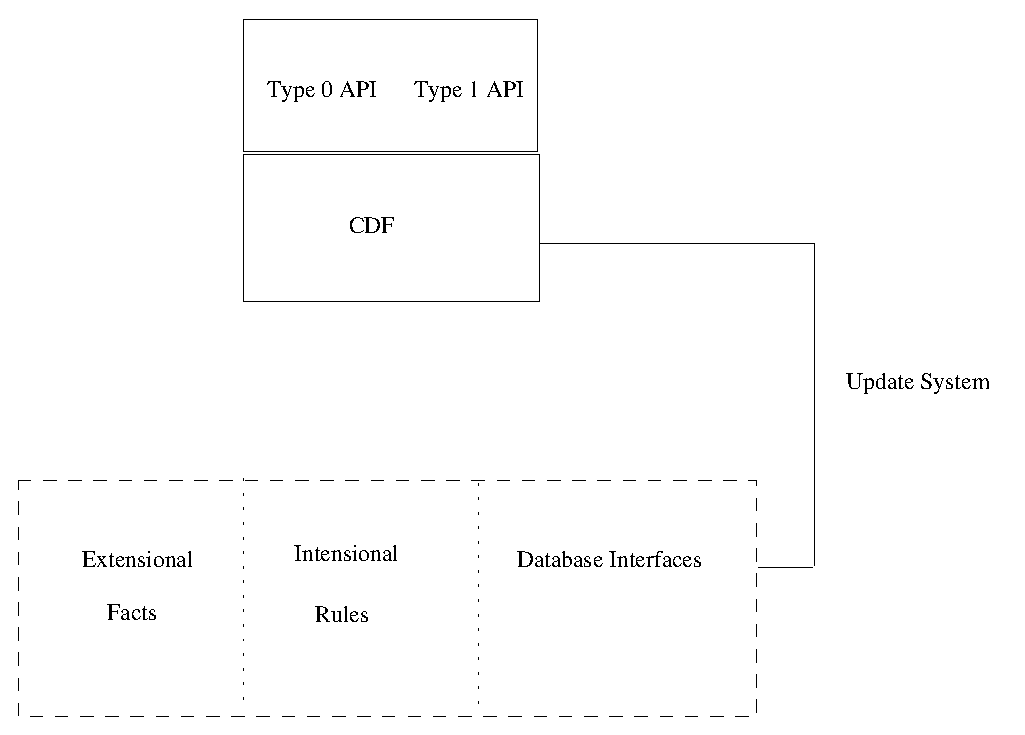
\epsfig{file=Figures/arch.eps,width=0.80\textwidth}}
\caption{A High-Level Architecture of CDF and XJ}
\label{fig:arch}
\end{figure}
%--------------

CDF instances can be classified either as Type-0 or a Type-1, each of
which has its own interface.  Type-0 instances are useful for storing
large amounts of information; and consistency and implication in
Type-0 instances is computable in polynomial time.  Type-0 instances
describe classes by existential and universal relations, qualified
number restrictions, and relational hierarchies, but descriptions omit
negation and disjunction. Type-0 instances also support a direct
product construction for objects and classes.  
\mycomment{
These product classes and objects can be useful for representing
certain types of non-binary relations, and are particularly useful for
incorporating knowledge represented as RDF facts \cite{}.  }
Information in Type-0 CDF instances is tightly coupled to XSB's
query mechanism, and CDF ensures that only the most specific answers
(according to a given inheritance hierarchy) are returned for any
Type-0 query.

Type-1 instances extend Type-0 instances to describe classes using
negation and disjunction, and thus permit descriptions that are
equivalent to an expressive description logic.  In fact, a Type-1 CDF
instance can be seen as a knowledge base in which various classes are
described via {\em class expressions}, which correspond to formulas in
description logics.  Reasoning in Type-1 instances is done via the CDF
theorem-prover.  Using the Type-1 API, users may ask whether a given
class or object is consistent, whether a given class expression is
consistent with a class or object; or whether a given class expression
is entailed by a given class or object.  The problems of determining
consistency or entailment of a Type-1 class expression have a high
degree of complexity.  To solve these problems the CDF theorem prover
uses several heuristics, but a determined (or unlucky) user can always
find class expressions that require a large amount of time to check.

Of course, ontology management systems require many features in
addition to reasoning and representation features \cite{MGPS03}.  We
mention some of these features.

\begin{itemize}
\item {\em A Semantic Checking System}.  CDF has various mechanisms for
ensuring consistency of objects and classes both at the Type-0 or
Type-1 level.  Various levels of consistency can be checked during
various operations on the CDF instance.
%
\item {\em A Component System}. Reusability of ontologies is supported
by the {\em component} structure of CDF.  An ontology component may be
maintained by separate users or organizations in different locations
and assembled in various ways by applications.
%
\item {\em A Concurrency System}. (Non open-source) Based on the
component structure, the {\em concurrency} mechanism for CDF allows
users to update their own CDF instances and to periodically update a
common store. Naturally, the various mechanisms in CDF for ensuring
consistency that are vital to ensuring coherency when users update
their systems concurrently.
%
\item {\em Database Interfaces}. (Non open-souce) CDF supports various
interfaces to databases so that CDF facts can be stored in a database
or mapped to database tables.
\end{itemize}

Based on these features, CDF can support user interfaces in a number
of ways.  One of the most convenient is to use a XSB/Java interface
such as InterProlog~\cite{Cale01} or JAXSB~(see
\texttt{http://xsb.sourceforge.net}) and then write a user interface in
Swing or some other Java Graphics library.  One of the easiest ways to
do this is to make use of the {\em XJ system} which allows Swing Gui
objects to be represented as Prolog terms (the XJ system is non
open-source) From a systems perspective, a graphical interface is then
written XJ library Swing widgets or specialized XJ-CDF Swing widgets.
CDF per-se has the following graphical packages and applications.
%
\begin{itemize}
%
\item {\em An XJ Caching System}. Adds and deletes to CDF are extended
with a notification mechanism so that Java Swing objects (created with
XJ, XSB's graphics system) reflect the state of CDF even when it
dynamically changes.
%
\item {\em A Visual Editor}. Finally,  CDF supports a graphical editor
that allows users both to visualize an ontology and to perform the
functions mentioned so far.
\end{itemize}
%
Extensional facts, intensional rules, updates, the Type-0 and Type-1
interfaces, consistency checking predicates and the full component
system are available as an open-source package for XSB.  Other
features, concurrency mechanisms, specialized database interfaces, XJ
support and the editor are not open-source.  The open-source code can
be obtained via \texttt{xsb.sourceforge.net}.  Inquiries about the full
Coherent Description System should be made to
\texttt{ode@xsb.com}.



